\documentclass[]{article}
%\usepackage{setspace}
%\onehalfspacing
\usepackage{amsmath,amssymb,amsthm}
\renewcommand{\qedsymbol}{$\blacksquare$}
\usepackage{amsmath}
\usepackage{amsfonts}
\usepackage{mathrsfs}
\usepackage{amssymb}
\usepackage{bm}
\usepackage{enumerate}
\usepackage{mdwlist}
\usepackage{dirtytalk}
\usepackage{xparse}
\usepackage{physics}
\usepackage[cmtip,all]{xy}
\newcommand{\longsquiggly}{\xymatrix{{}\ar@{~>}[r]&{}}}
\usepackage{pdfpages}
\usepackage{graphicx}
\usepackage{xcolor}% http://ctan.org/pkg/xcolor
\usepackage{hyperref}% http://ctan.org/pkg/hyperref
\hypersetup{
  colorlinks=true,
  linkcolor=blue!50!red,
  urlcolor=green!70!black
}
\setcounter{MaxMatrixCols}{13}
\setlength\parindent{0pt}
\usepackage[none]{hyphenat}
\usepackage[hmarginratio=1:1]{geometry}
\begin{document}

{\Large Physics 614 Homework 7}\\
{Jeremy Welsh-Kavan}\\
\hfill \\
\noindent\rule{15cm}{0.4pt} \\


\begin{enumerate}[1.]


\item {\bf Gibbs free energy of the van der Waals gas} \\


\begin{enumerate}[i.]
 
\item The Helmholtz free energy of the van der Waals gas has the form \\

\begin{equation}
\begin{aligned}
F(T,V,N) & = - N k_B T \ln(  \frac{V}{N} - b ) - \frac{ N^2 a }{V} + N f(T) \\
\end{aligned}
\end{equation} \\

for some function $f$. Recall, the Helmholtz free energy and the Gibbs free energy are related via \\


\begin{equation}
\begin{aligned}
G & = F + PV \\
\end{aligned}
\end{equation} \\

So we can write $G$ as

\begin{equation}
\begin{aligned}
G(P,T,N,V) & = - N k_B T \ln(  \frac{V}{N} - b ) - \frac{ N^2 a }{V} + N f(T)  + PV \\
\end{aligned}
\end{equation} \\

Dividing by $N$ to get the chemical potential per particle, we have \\

\begin{equation}
\begin{aligned}
\mu (P, T ; v)  & = -  k_B T \ln( v - b ) - \frac{ a }{v}  + Pv  +  f(T)  \\
\end{aligned}
\end{equation} \\
 
where $v = V/N$.  \\


\item Dropping $f$ from Eq. (4), and differentiation with respect to $v$ to minimize $\mu$ gives \\

\begin{equation}
\begin{aligned}
\pdv{ \mu }{ v} & = -  k_B T\frac{1}{  v - b } + \frac{ a }{v^2}  + P  \\
0 & = -  k_B T\frac{1}{  v - b } + \frac{ a }{v^2}  + P  \\
\implies P + \frac{ a }{v^2} & =  k_B T\frac{1}{  v - b } \\
\end{aligned}
\end{equation} \\

which is indeed the Van der Waals equation of state. \\


\item Define the dimensionless variables, $g := \mu /k_B T$, $p := P/p_c$, $\nu := v/v_c$, and $t := T/T_c$, where $T_c, P_c$, and $v_c$ are the values of the corresponding variables at the critical point. From the lecture notes, we know that $k_B T_c = 8a/27b$, $p_c = a/27b^2$, and $v_c = 3b$. Substituting these values in Eq. (4) yields

\begin{equation}
\begin{aligned}
\mu (P, T ; v)  & = -  k_B T \ln( v - b ) - \frac{ a }{v}  + Pv   \\
\longsquiggly \frac{ \mu (P, T ; v)    }{ k_B T_c } & = - t \ln( 3b \nu - b ) - \frac{  27 b  }{ 8a  } \frac{ a }{ 3b \nu }  + \frac{  27 b  }{ 8a  }  \frac{ a  }{ 27 b^2  }  p 3b \nu \\
g( p , t; \nu) & = - t \ln( 3 \nu - 1 ) - \frac{  9   }{ 8 \nu  } + \frac{ 3 p \nu  }{ 8  }   \\
\end{aligned}
\end{equation} \\

where the term which did not depend on $p$ or $\nu$ has been dropped. \\

\item On the next page is a plot of $g(\nu)$ for $p = 1.4$ and $t$ taking a range of values. Each curve has at most one minimum which corresponds to the existence of an inflection point on the plot of the Van der Waals gas in the $PT$-plane. \\

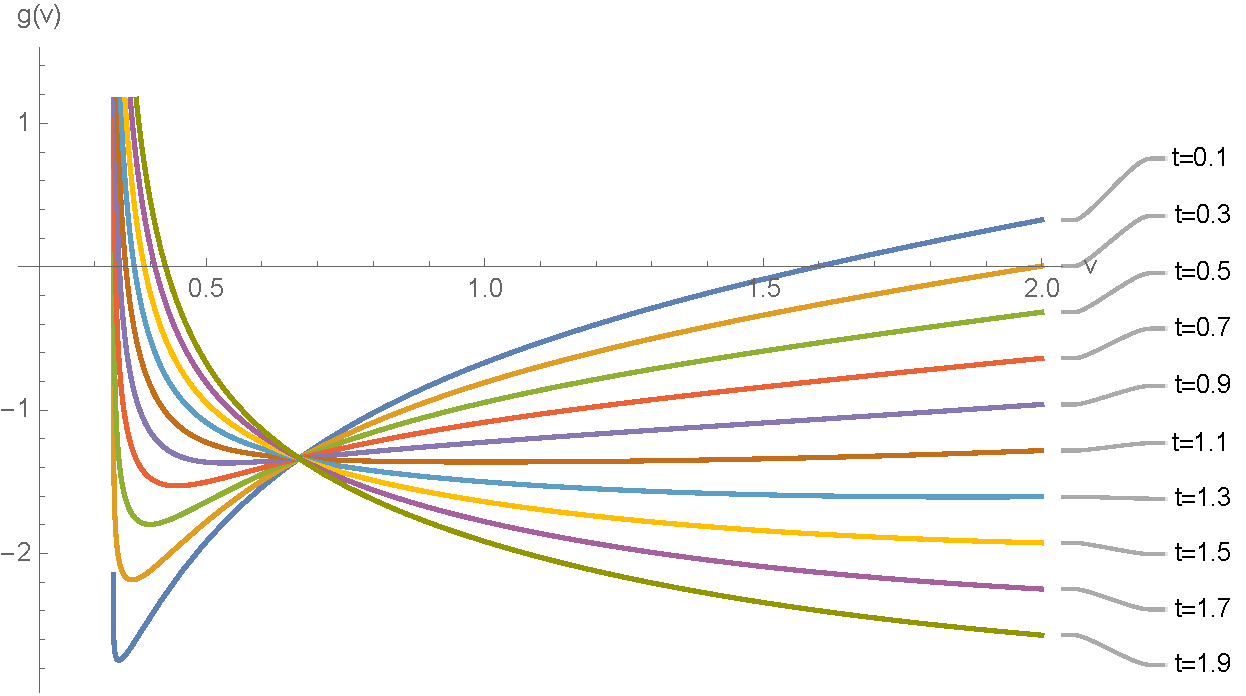
\includepdf[pages=1]{g_v_plot2.pdf}

\item Below is a similar plot but for $p=0.6$ and over a smaller range so that we can estimate the value of $t$, for which the phase transition from gas to liquid occurs, more precisely. This seems to occur at approximately $t = 1.05$. 

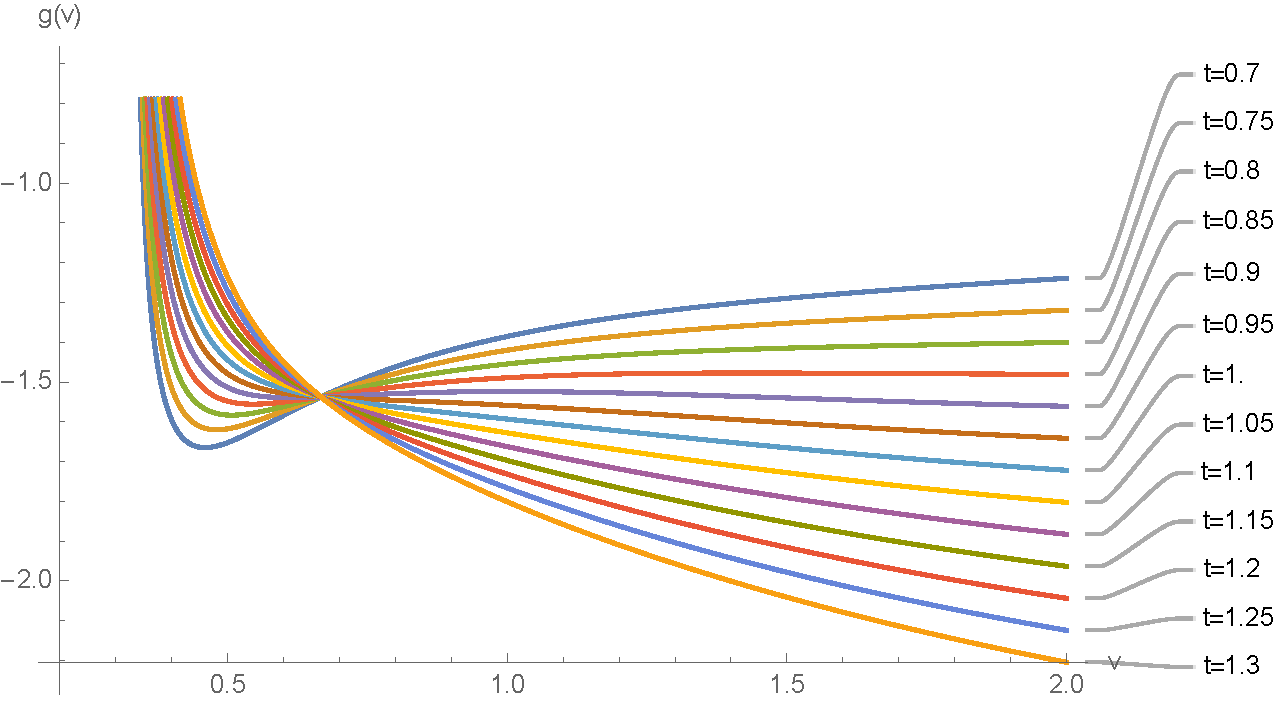
\includepdf[pages=1]{g_v_c_plot.pdf}


\end{enumerate}

\noindent\rule{15cm}{0.4pt} \\

\item {\bf Dieterici equation of state} \\

We consider a gas whose equation of state is

\begin{equation}
\begin{aligned}
P & = \frac{  k_B T }{ v- b } \exp(  - \frac{ a }{ k_B T v } ) \\
\end{aligned}
\end{equation} \\

\begin{enumerate}[i.]

\item This is where profound apathy set in and I decided I was happy taking the proverbial ``L" on this assignment. Apologies for the boring assignment submission. \\

Below is a plot of $P(v)$ for several values of $k_B T$. The plots with vertical asymptotes are of $P(v)$ with $a = 1$ and $b = 1$, while the plots with maxima are with $a = 1$ and $b = 0.1$. This suggests that the critical behavior of this gas is more dependent of $a$ and $b$ than on $T$. One would like to find a condition on $a$ and $b$ such that $P(v)$ experiences a gas-liquid phase transition. This might be found by requiring that, for some $T$, $\partial P/ \partial v = $ and $\partial^2 P/ \partial v^2 = 0$. 










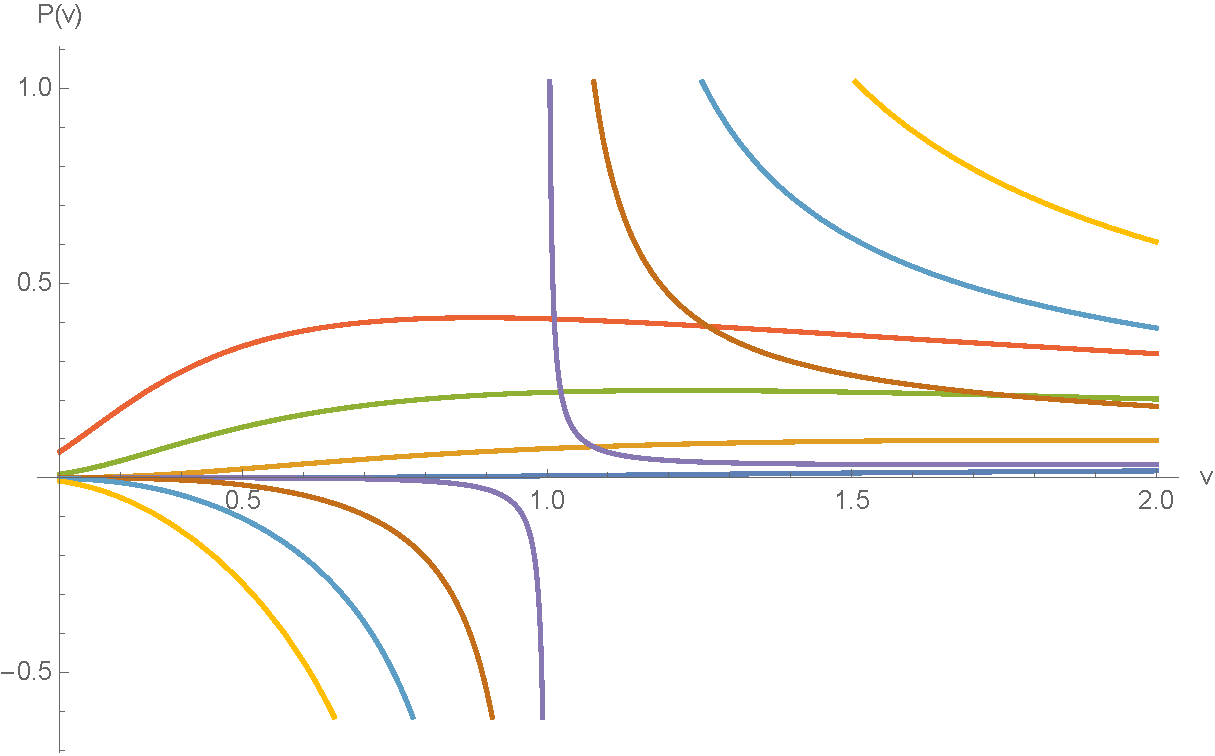
\includepdf[pages=1]{p_stop.pdf}




\end{enumerate}





\newpage




\end{enumerate}


 
\noindent\rule{15cm}{0.4pt} \\

$$\clubsuit$$

\end{document}











%\begin{equation}
%\begin{split}
%\end{split}
%\end{equation}
